195. \begin{figure}[ht!]
\center{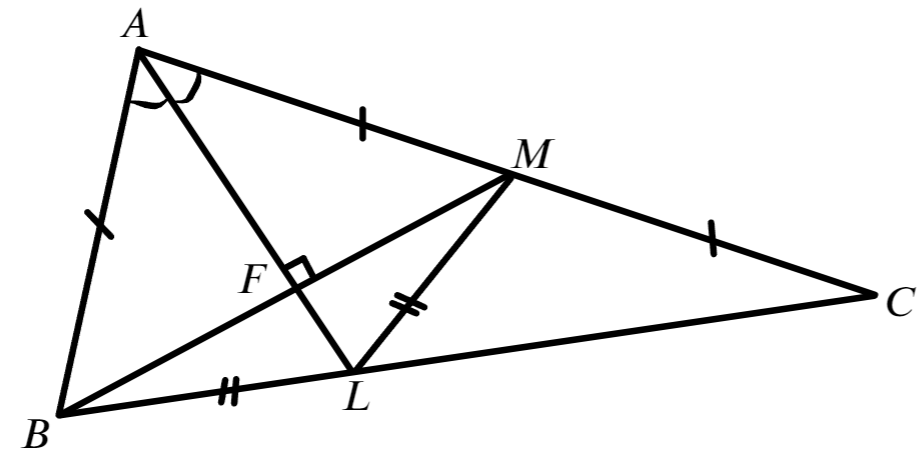
\includegraphics[scale=0.35]{g9-195.png}}
\end{figure}\\
Пусть $AL$ и $BM$ пересекаются в точке $F.$ В треугольнике $ABM$ биссектриса $BF$ совпала с высотой, значит он равнобедренный и $AB=BM,\ BF=FM.$ Тогда аналогично равнобедренным является и треугольник $BML$ (высота совпала с медианой), значит $AM=AB=\sqrt{3},\ BL=ML=1.$ По свойству основания биссектрисы имеем соотношение
$\cfrac{BL}{LC}=\cfrac{AB}{AC},\ \cfrac{1}{LC}=\cfrac{1}{2},$ откуда $LC=2.$ Тогда в треугольнике $ABC$ выполняется равенство $AB^2+BC^2=3+(1+2)^2=12=(2\sqrt{3})^2=AC^2,$ поэтому он является прямоугольным и его площадь равна $\cfrac{3\sqrt{3}}{2}.$\\
